\chapter{Analysis of Power Consumption Dataset}

In recent years, we observe widespread IoT technologies in everyday life due to the decreasing price of smart sensors and high-quality network availability. Electricity distribution and consumption are no different, and smart electric meters are now standard components in modern households. It eventually leads to a large amount of sensor data structured as a time series, and there is a need for efficient analysis tools. As a part of our research in Gauss Algorithmic, we got a task to analyze such a dataset. Our assignment is to analyze this dataset and detect customers with potentially abnormal behavior.

This chapter will go through all steps necessary to analyze this dataset using the techniques mentioned in previous chapters.

\section{Dataset}
The first step is a detailed overview of the dataset. Our dataset consists of a large set of power consumption curves for customers located in Slovakia. Because of the strong emphasis on customers' privacy, all data are completely anonymous. We have only randomly generated numbers from our contracting authority as labels and power consumption curves for every consumer. Thus, we lack information about the customer's location or type (apartment, household, company).
\begin{figure}[htp]
    \centering
    \includesvg[width=\textwidth]{img/dataset-example.svg}
    \caption{Example of power consumption curves with missing values and significantly different behavior.}
    \label{fig:dataset-example}
\end{figure}
We have over 20~000 time series from the February 1st 2017 to August 1st 2018. The sampling rate of our time series is one value every 15 minutes. After the initial analysis, we found that there is a high rate of incorrect or missing data. There are entirely missing days throughout the period and even several months in 2018. On average, we have approximately 52~000 data points, which corresponds to almost 547 days for each customer.

\section{Requirements}

With our dataset's detailed overlook, we will divide our work into two objectives to accomplish our assignment. The first is to process the dataset into a form that could be easily analyzed, and the second is the analysis and anomaly detection.

\begin{enumerate}
    \item A combination of rapidly changing customer power consumption, sensor errors, changes based on external factors, and lack of information about a customer makes this task remarkably challenging. Another critical detail is the size of our dataset and the length of individual time series. To explore and analyze this data, we have to prepare the following steps: propose preprocessing and feature extraction resistant to missing data, analyze long-term behavior, maintain reasonable time and space complexity for all steps.
    \item After the data preparation, we want to analyze our dataset and find outliers. As we are working with a large dataset of time series, we want to prepare meaningful views and visualizations, which will guide a user towards clusters and anomalous data.
\end{enumerate}


\section{Preprocessing}
We are working with a large number of data from smart electric meters. It is not unusual to encounter missing or unrealistic values due to sensor or network error. It is essential to preprocess this type of defects, so they will not interfere with further analysis.

We define two unrealistic value cases: values with negative power consumption and sudden dramatic change in power consumption only for one data point. It is not uncommon to observe a combination of both. We assume that this type of error is due to sensor or network failure. To deal with values below zero, we replace them with missing values. To remove value jumps, we compute our power curve's second derivation and replace values with a disproportionately large absolute value of the second derivation by missing values.

We are not replacing the missing values in our preprocessing step. Instead, we use the feature extraction technique that is resistant to them. We will address this problem more in the next section.

\section{Feature Extraction}
Consumers' power consumption tends to change rapidly due to the sudden extensive usage of electric devices, yet it should be more stable in the long-term. Thus we want to extract features that will not be significantly affected by them. These features will provide a better overview of user behavior and make it possible to find users with a similar one. To overcome fluctuations in short periods, we want to study long-term periodic and non-periodic behavior. We do this by extracting seasonalities (periodic behavior) and trends (non-periodic behavior) in customer power consumption.

Due to the geological location and climate in Slovakia, power consumption is generally changing during the year. The main factors are changes in temperature and sunlight hours through seasons. To capture these changes, we extract weekly seasonality separately for every meteorological season. Another characteristic comes from daily seasonality, where we distinguish between free days and workdays. We also want to utilize trends and yearly seasonalities of our data. As holidays have a substantial impact on power consumption, we want to capture their effect in the model.

For extracting these seasonalities and trends from our data, we are using the Prophet by Facebook \cite{exp:FbProphet}. It uses a decomposable time series model with three main components: trend, seasonality, and holidays \cite{exp:lin-model}. Formally defined as:
\begin{equation}
    y(t) = g(t) + s(t) + h(t) + \epsilon_t    
\end{equation}
Where $g(t)$ is the trend function, $s(t)$ is the seasonality function, $h(t)$ corresponds to the effects of holidays, and $\epsilon_t$ is noise keeping the normal distribution.

Prophet provides an interface to detect changepoints in trends automatically. However, because our data are relatively short, only one and a half years of data, we do not expect any significant trend changes in our data. Thus we are using a linear trend with zero change points. The Prophet uses the Fourier series representation to model multiple periodic effects (seasonalities) with different lengths. We use yearly seasonality, free day and workday daily seasonality, and weekly seasonality for every meteorological season. To include the effects of holidays, it uses a matrix of regressors corresponding to every holiday. This effect is also applied to the surrounding days. Other essential features are the ability to deal with missing values, speed, and scalability.
\begin{figure}[h]
    \centering
    \includesvg[width=0.88\textwidth]{img/seasonalities.svg}
    \caption{Example of seasonalities extracted using the Prophet.}
    \label{fig:seasonalities}
\end{figure}

In this work, we are manually defining seasonalities based on the expected behavior of the different customer types for our use case. First, we expect a different behavior on free days (holidays, weekends) and workdays. Then because of the changes in weather during a year, there can be a change in weekly behavior, so we are using a weekly seasonality for every season. Finally, we want to see the trend and the yearly seasonality. We can see the example of this decomposition in Fig.~\ref{fig:seasonalities}. Using this feature extraction allows us to find customers with similar properties in one seasonality but significantly different behavior in others -- for example, two customers with almost identical seasonalities yet significantly higher power consumption which could be a sign of energy theft.

In summary, we are describing our original time series with eight new time series: free day and workday seasonalities, spring, summer, winter, and autumn weekly seasonalities, yearly seasonality, and trend. In the next section, we will provide techniques to work with such multi-model data.

\section{Interactive Feature Space Building}
Once we use seasonalities and trends, our dataset changes from univariate time series into a multi-model time series of eight time series of different lengths. In combination with a lack of knowledge about the customer, we have a large unsupervised multi-model dataset. We will split our solution into two parts: multi-model data and dataset size.

\subsection{Multi-Model Prototyped Feature DTW Transformations}
We propose the Multi-model Prototyped Feature DTW transformations (MPFDTW) to work with the multi-model model time series dataset. As Kate has shown, it is possible combining multiple Feature DTW transformations (FDTW) \cite{met:fDTW}. Similarly to his approach, the MPFDTW is a union of FDTW transformation for every component (model) of our multi-model time series. Having a dataset $S = {T_0, T_1, \dots, T_n}$ of multi-model time series $T_n = (a_{n0}, a_{n1}, \dots, a_{nj})$ where $a_nj$ are time series of arbitrary length and $A_j = (a_{0j}, a_{1j}, \dots, a_{nj})$ are tuples of time series from one model (dimension), we define the MPFDTW transformation as:
\begin{equation}
 MPFDTW(S) = ( FDTW(A_{0}) | FDTW(A_{1}) | \dots | FDTW(A_{j}) )
\end{equation}

While defining the MPFDTW as an aggregation of FDTW as an underlying transformation, we can use the prototype version of FDTW to reduce the time and space complexity. Iwana et al. proposed two ways for the prototype selection from the full distance matrix for the dataset \cite{met:protofDTW}. The first one is to use statistics to remove statistically insignificant feature vectors, and the second one to use the AdaBoost algorithm to select the best features for classification. Even though the first method is usable on unsupervised problems, it uses the full distance matrix, making it unpractical on large datasets.

\subsection{Prototype Selection}
The prototypes are crucial for the success of our transformation, but their correct selection is a challenging task. Once we have a feature vector from the prototype, we can check how significant it is in our model, how much it correlates with other feature vectors or any different quality measures.  However, as there is no proper way to compare the quality of the prototype before we compute the feature vector from it. We propose several bottom-up methods for the prototype selection:
\begin{enumerate}
    \item Random selection
    \item Manual selection
    \item Selection by density
    \item Selection by Predicted Correlation
\end{enumerate}

\subsubsection{Random Selection}
The first and most straightforward option is to use randomly selected prototypes. This approach is very efficient, and if our sample is large enough, we are covering a good portion of the full feature space. Based on our tests on the UCR datasets, a random prototype selection seems to be a very efficient approach that still produces comparable results in terms of classification accuracy (Appendix~\ref{sec:app-ucr}). Because of these advantages, we recommend using this method of prototype selection as a starting point.

\subsubsection{Manual Selection}
The second approach is selecting specific time series as prototypes by hand. It is usable if the user has deep knowledge about the data and could pinpoint the significant time series. As the resulting feature vectors are the distances to these specific time series, it is easily interpretable for the user.

Even though this method has an excellent explainability, the user could miss some important time series, either by selecting correct examples or selecting time series relevant from individual but no computational point of view. We recommend combining this approach with randomly selected prototypes and comparing the feature importance of individual feature vectors because of these potential issues.

\subsubsection{Selection by Density}
Another approach comes from an observation that we need more points to describe a dense region than the sparse one, similar to the Kohonen map \cite{exp:Kohonen1982}. This strategy starts with a random sample and then uses data visualization to select new prototypes from the dense regions and removing prototypes that are far away.

Because after the MPFDTW transformation, the transformed feature matrix has the number of dimensions equal to the number of selected prototypes, we can encounter the Curse of Dimensionality \cite{exp:curse-of-dim}. This is problematic for density-based techniques. Because there is no conventional solution to this issue, instead of using a fully automatic solution, we use a combination of dimensionality reduction and visualization techniques. Based on the work with our dataset, this approach yields stable results.

\subsubsection{Selection by Predicted Correlation}
As two strongly correlated feature vectors do not give much information, the last strategy we propose comes from an assumption that we could predict the correlation of feature vectors from other time series from information about current prototypes. 

We start with the random prototype selection and transform the dataset into a feature matrix. Then we use Spearman's rank correlation coefficient and compute the correlation matrix between the feature vectors produced from our prototypes. Afterwards, we use the feature matrix and correlation coefficient of other prototypes to train a regressor to predict the correlation on other time series for each prototype. Finally, we select the prototypes with the lowest average predicted correlation (Appendix~\ref{sec:app-corr}).


\subsection{Interactive Feature Space Building}
Considering the techniques used for prototype selection, we split our feature space building process into an interactive iterative pipeline. The pipeline consists of seven steps:
\begin{enumerate}
    \item Select a subsample of the dataset.
    \item Build a Prototyped Feature DTW space.
    \item Vizualize the dataset.
    \item Choose new or remove prototypes using the visualization.
    \item Repeat steps 2-4 until we are satisfied with the result or do not see any change.
    \item Apply MPFDTW to the whole dataset.
\end{enumerate}

Because our dataset consists of a large number of multi-model time series, we will randomly select a fraction of our dataset in the first step. This allows us to work with the data in real-time. We are using the subsample only for the initial iterative feature space building. These steps require human input, and very like we have to them several times before we are satisfied with the result.

In the second step, we are building the new feature space by using MDFDTW. As we have no information at the start, in the first iteration, we are using the randomly selected subsample as the initial selection of prototypes. Based on our test on the UCR datasets, a random prototype selection seems to be a very efficient approach that still produces comparable results in terms of classification accuracy (Appendix ~\ref{sec:appendix}). After the first iteration, the feature space building is fully automatic based on the prototypes selected or removed in step three. As we are using the iterative approach, we do not compute already computed feature vectors, increasing the efficiency.
\begin{figure}[htp]
    \centering
    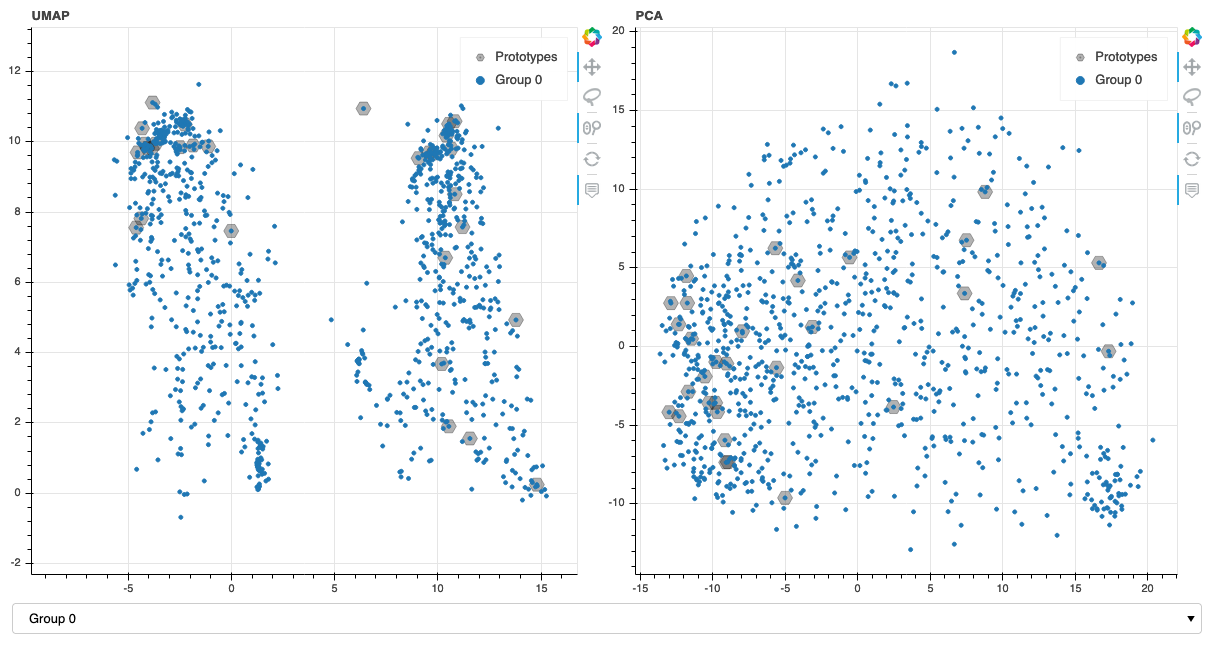
\includegraphics[width=0.9\textwidth]{img/prototypes.png}
    \caption{Visualization of the Power Consumption dataset using the PCA and UMAP. Prototypes are highlighted by grey hexagon.}
    \label{fig:prototypes}
\end{figure}

Afterward, we prepare multiple data visualizations for dataset analysis. Firstly, we use PCA and UMAP/densMAP to visualize our dataset's global and local structures. As displayed in Fig~\ref{fig:prototypes}, we can study the local and global structure of the dataset, including prototypes' positions. Using interactive zoom and selection, we can select time series to inspect them directly, study their position and surrounding in the UMAP and PCA transformations, and closely examine their seasonalities and trends (Fig.~\ref{fig:selected-seasonalities}).
\begin{figure}[htp]
    \centering
    \includesvg[width=0.85\textwidth]{img/selected-seasonalities.svg}
    \caption{Inspection of trends and seasonalities.}
    \label{fig:selected-seasonalities}
\end{figure}

To help with the inspection, we are providing multiple coloring options. Firstly, it is possible to select, group, and color time series manually (Fig.~\ref{fig:coloring}). As this coloring is persistent throughout iterations, we can use it to study the change of positions of our time series in terms of their surroundings. Other options are to use coloring by automatic clustering or anomaly detection score. We will discuss this in the next section.
\begin{figure}[htp]
    \centering
    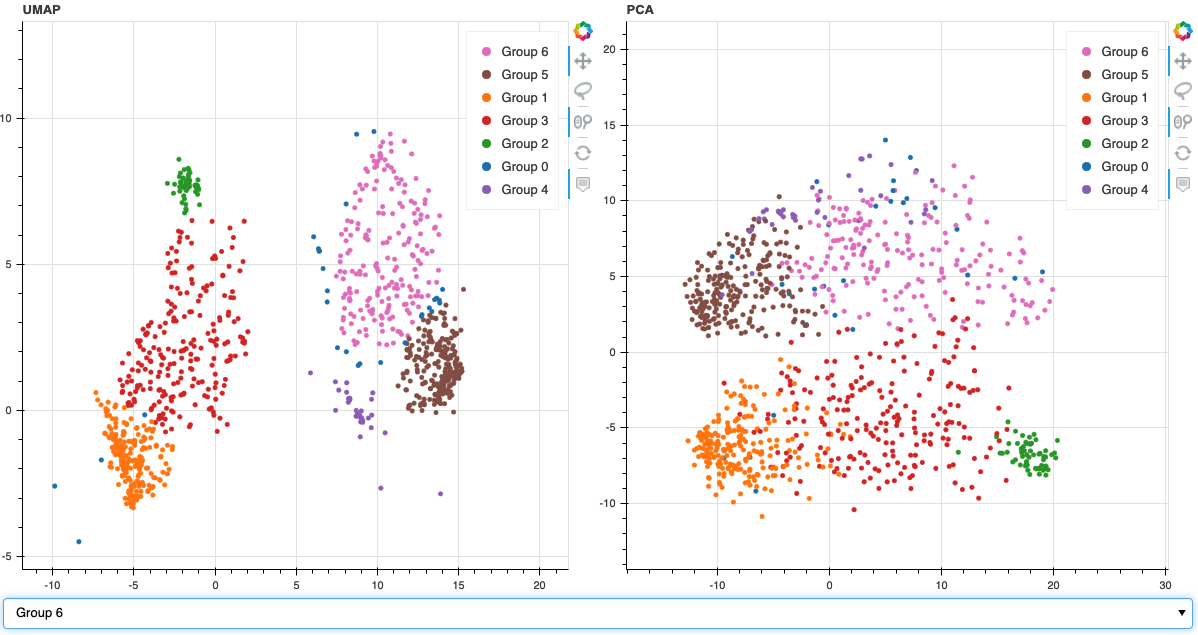
\includegraphics[width=0.9\textwidth]{img/overview.png}
    \caption{Manual separation of time series into groups that are persistent during iterations.}
    \label{fig:coloring}
\end{figure}

\section{Clustering and Anomaly Detection}
As our data are transformed into a feature matrix, we can practically use any clustering algorithm for spatial data. In our application, a user can choose from all methods available in \textit{Scikit-learn} or \textit{HDBSCAN}. To overcome the curse of dimensionality from MPFDTW transformation and to reduce the computational time, we are using two clustering pipelines:
\begin{enumerate}
    \item We are using \textit{PCA} to reduce the number of dimensions into 100-50 dimensions based on the explained variance ratio for \textit{distance-based} clustering methods. Even though these clustering methods are not as affected by high dimensionality as \textit{density-based} methods, they usually perform better on lower dimensions.
    \item For \textit{density-based} methods \textit{OPTICS} and \textit{HDBSCAN}, we use PCA transformation into 50 dimensions followed by UMAP/densMAP embedding into 30 dimensions. As these embeddings preserve the local structure in the data, they help to overcome the sparsity of high-dimensional space.
\end{enumerate}

After the clustering, we can visualize the results in the original visualization of our dataset. It is possible to study the clusters in a detailed view or use them to discover new prototypes for next iterations.

For detecting the anomalies in our dataset, we are using \textit{Isolation Forest} and \textit{LODA}. It is possible to use them on a whole dataset or a selected subsample. As both these methods are very efficient, we use them directly on the MPFDTW feature vector without any dimensionality reduction. Another option for anomaly detection comes from clustering with OPTICS or HDBSCAN as both methods select certain points as noise. Similarly to the clustering, we can plot the results of anomaly detection in our data views to either study their location within the dataset or to use them for identifying new potential prototypes.


\section{Implementation}
Our solution is mainly usable by data scientists, so we tried to use the typical technical stack in this field. We are using the Python programming language, and our solution is distributed as a single open-source package.

We implemented the Feature DTW and related algorithms using the well-known API defined by the \textit{Scikit-learn} project \cite{exp:sklearn_api,exp:scikit-learn}, which is the most used tool for machine learning in Python. As \textit{Scikit-learn} does not natively support work with time series, we stick to the time series interface defined by the \textit{Tslearn} library \cite{exp:tslearn}.

Based on our knowledge of data science work, the most significant part is in the \textit{IPython} \cite{exp:ipython} and \textit{Jupyter notebooks} \cite{exp:jupyter}, and so our implementation is fully integrated into these technologies. For the visualization and rendering, we use a combination of \textit{Matplotlib} package \cite{exp:matplotlib} for smaller non-interactive visualizations, \textit{Bokeh} server \cite{exp:bokeh} for interactive visualizations, and the \textit{Datashader} \cite{vis:datashader} for processing and rendering the large time series.

Even though there are some implementations of the LODA anomaly detection method, none of them are complete, and all of them lack the feature to explain the cause of the anomaly. We prepared an open-source \textit{anlearn} anomaly detection python package \footnote{\url{https://github.com/gaussalgo/anlearn}} with our implementation of LODA, that is, towards our knowledge, the only one containing sparse projections and the ability to explain cause of the anomaly.

As we want our work to be fully replicable, we are using the \textit{Nix} package manager \cite{exp:dolstra2008nixos} in combination with pinned requirements for all Python packages and their dependencies. This allows us to have a fully replicable work environment with the exact version of Python and all the used packages.

We were using only open-source packages in our work, and all of our source codes, including all notebooks from experiments, are available at our Github repository \footnote{\url{https://github.com/H00N24/visual-analysis-of-big-time-series-datasets}}.

\section{Results}

\section{Chapter Summary}
In this chapter we proposed a 